\documentclass{article}
\usepackage{amsmath,amssymb}
\usepackage{tikz}
\usetikzlibrary{arrows.meta,positioning,calc,shapes.geometric}
\pagestyle{empty}
\begin{document}
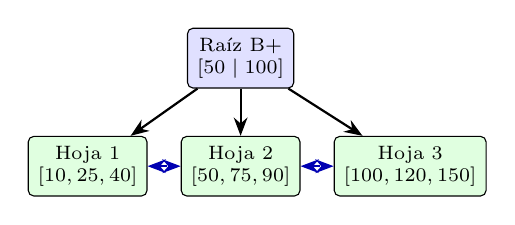
\begin{tikzpicture}
\tikzset{node distance=0.6cm and 0.5cm, every node/.style={font=\scriptsize, draw, rounded corners=2pt, align=center, inner sep=3.5pt}}
\node (root) [fill=blue!12] {Raíz B+\\$[50 \mid 100]$};
\node (l1) [below left=of root, fill=green!12] {Hoja 1\\$[10, 25, 40]$};
\node (l2) [below=of root, fill=green!12] {Hoja 2\\$[50, 75, 90]$};
\node (l3) [below right=of root, fill=green!12] {Hoja 3\\$[100, 120, 150]$};
\draw[-Stealth, thick] (root) -- (l1);
\draw[-Stealth, thick] (root) -- (l2);
\draw[-Stealth, thick] (root) -- (l3);
\draw[Stealth-Stealth, dashed, thick, blue!70!black] (l1) -- (l2);
\draw[Stealth-Stealth, dashed, thick, blue!70!black] (l2) -- (l3);
\end{tikzpicture}
\end{document}
